\documentclass[12pt]{article}

\title{Side Project Summary 2017--2019}
\author{William John Holden}
\date{\today}

\usepackage{amsmath,amsthm}
\usepackage{mathtools}
\usepackage{parskip}
\usepackage{amssymb}
\usepackage[margin=1.0in]{geometry}
\usepackage{minted}
\usepackage[utf8x]{inputenc}
\usepackage[hyphens]{url}
\usepackage[hidelinks]{hyperref}
\usepackage{listings}
\lstset{basicstyle=\ttfamily,columns=flexible,frame=single,breaklines=true}
\usepackage{graphicx}

\begin{document}
\maketitle

\begin{abstract}
At 2017--2019 job I worked on several side projects.
I hope that these programs will be useful to others after I leave.
This document catalogs the purpose, capability, and usage of each program.
Only projects that were written directly in support of my job are listed here.
None of these programs require privileged access or installation, although host-based firewalls may interfere with network-aware programs.
\end{abstract}

\tableofcontents

\section{Connection Map} \label{sec:ConnectionMap}

\textbf{Location}: \url{https://github.com/wjholden/Connection-Map}

\textbf{Input}: Syslog messages on UDP port 514 from a Cisco ASA.

\textbf{Output}: World map with TCP/UDP connections plotted to their estimated geographical location (see figure \ref{fig:connection-map}).

\textbf{Language}: Java

\begin{figure}[h]
\centering
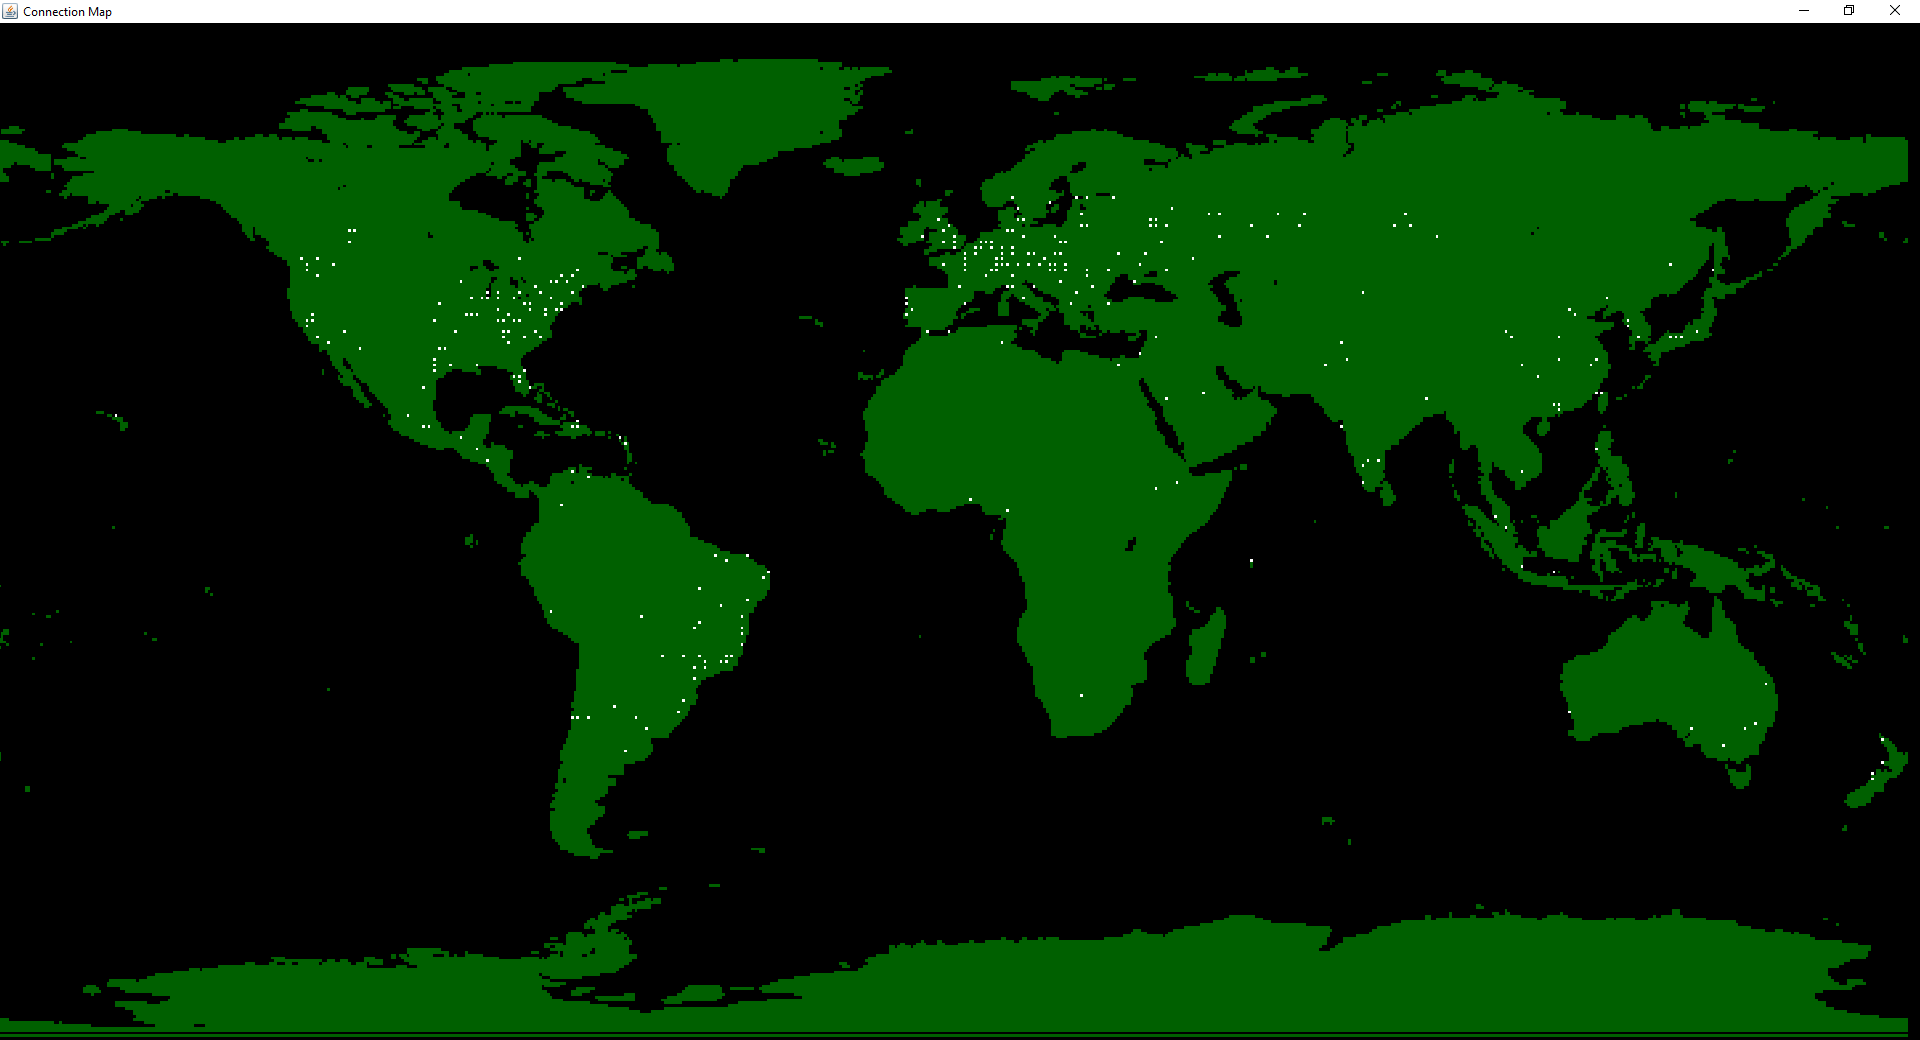
\includegraphics[width=\textwidth]{Connection-Map}
\caption{Connection Map}
\label{fig:connection-map}
\end{figure}

Connection Map is a Java 8 program to visualize network connections through a Cisco ASA firewall on a map. It uses the GeoLite2 ``GeoIP'' database available from \url{https://www.maxmind.com}.

Download the entire project from GitHub with the ``Clone or download'' button and select ``Download ZIP.'' Execute the runnable JAR at \texttt{Connection-Map/Connection\_Map.jar}. The \texttt{Connection-Map/lib/} folder contains all necessary dependencies. Press \texttt{h} for ``help'' inside the program.

Connection Map passively listens on UDP port 514 for Syslog messages. The program actually opens UDP port 514 as a multicast on the non-standard group \texttt{239.5.1.4}. Connection Map does not allow the operator to select which network interface it will bind to; binding decisions are left to the operating system. Microsoft Windows may bind the socket to an unexpected network interface. Use the command \texttt{netsh interface ipv4 show join} to observe which network interface the socket bound to. Npcap (included with Wireshark) may install a \texttt{Npcap Loopback Adapter} interface and VMware may install a \texttt{VMnet1} interface. These interfaces may have a faster ``speed'' and therefore lower route metric than the physical Ethernet and Wi-Fi interfaces (see \url{https://github.com/nmap/nmap/issues/1605}). If \texttt{netsh interface ipv4 show join} shows that \texttt{239.5.1.4} is joined on the incorrect interface, try disabling the other interface or change its metric (\texttt{Set-NetRoute}).

To configure a Cisco ASA to send Syslog messages to the Connection Map monitoring station, simply input the following commands in global configuration mode:

\begin{lstlisting}
logging enable
logging trap debugging
logging host inside x.x.x.x
\end{lstlisting}

\texttt{x.x.x.x} is either the unicast IP address of the monitoring station or \texttt{239.5.1.4}. The Connection Map program uses regular expressions to find Syslog messages 302013, 302014, 302015, and 302016 (see \url{https://www.cisco.com/c/en/us/td/docs/security/asa/syslog/b_syslog/syslogs3.html}). It assumes the external interface is named \texttt{outside} (case-sensitive). The name of the external interface is not configurable; if the name of the internal interface is not \texttt{outside} then the source code must be modified.

This program may be compatible with Cisco Firepower (see \url{https://www.cisco.com/c/en/us/td/docs/security/firepower/Syslogs/b_fptd_syslog_guide/syslogs3.html}).

Connection Map has limited utility in practice. This program is primarily ``eye candy'' for network operations centers, but it could be useful to give network operators a general sense of traffic patterns. For example, suppose a large organization has a data center on each continent. If a contenental data center in, say, Japan began servicing an unusually large number of clients in North America, then this could indicate an availability or routing problem.

\section{Route Monitor}

\textbf{Location}: \url{https://github.com/wjholden/Route-Monitor}

\textbf{Input}: One or more network addresses, subnet masks, and network descriptions as space-separated command-line arguments. Network descriptions may contain spaces if the entire description is surrounded witih quotation marks.

\textbf{Output}: A graphical panel of squares showing route advertisements (see figure \ref{fig:Route-Monitor-1}) and a textual representation of routes learned or removed on standard output.

\textbf{Language}: Java

\begin{figure}[h]
\centering
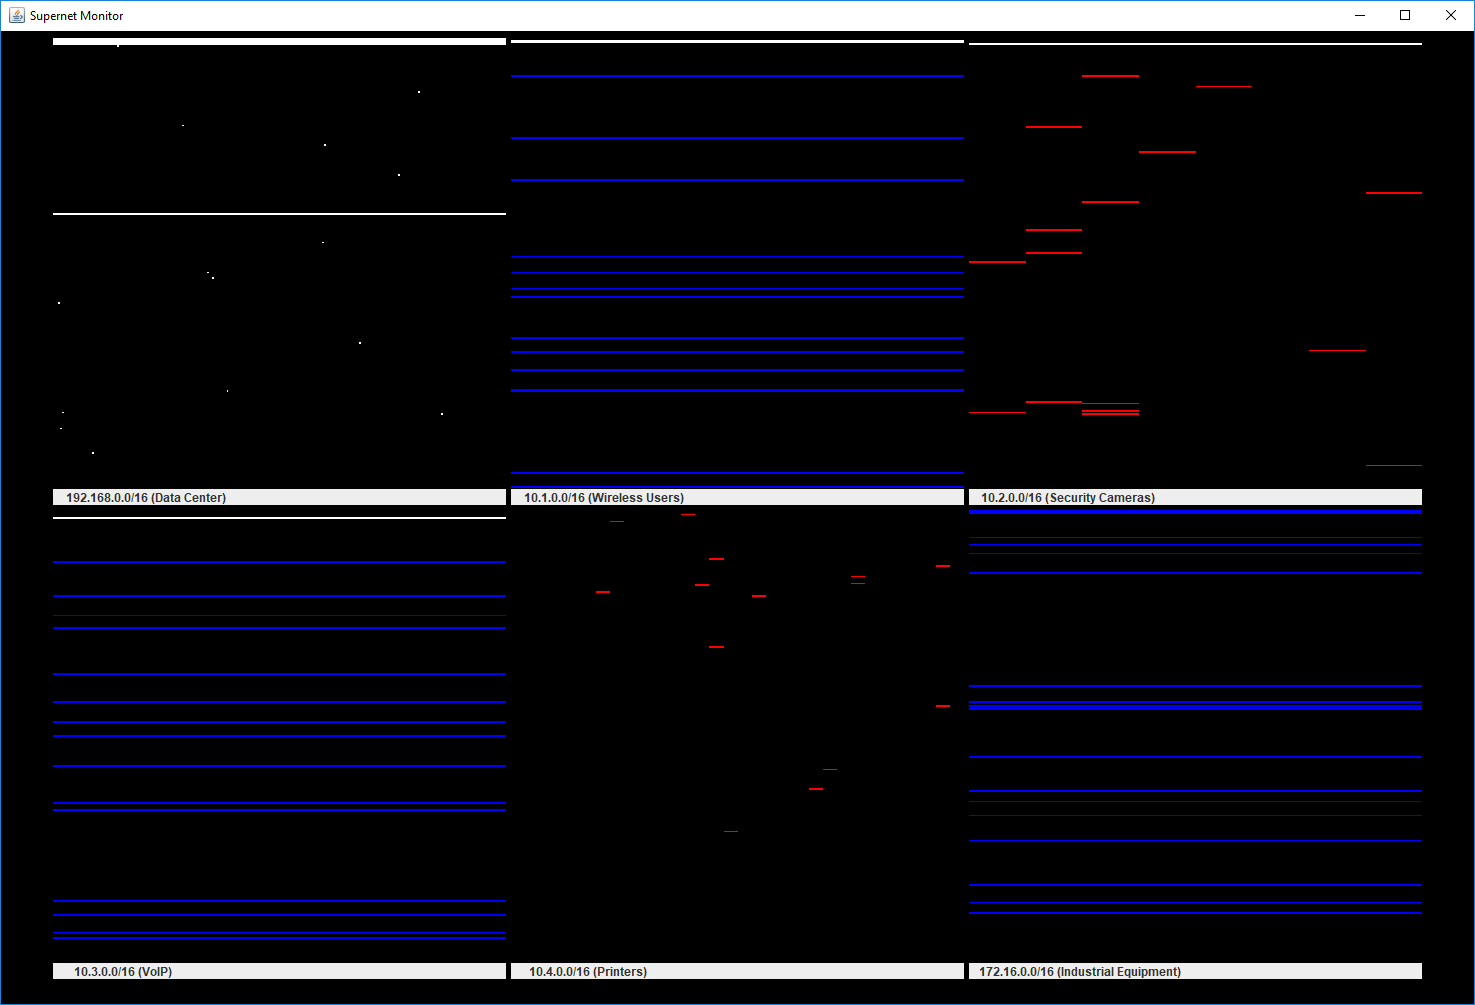
\includegraphics[width=\textwidth]{Route-Monitor-1}
\caption{Route Monitor}
\label{fig:Route-Monitor-1}
\end{figure}

Route Monitor builds upon a novel approach for visualizing route advertisements. Suppose a network operator wished to determine which subnets of \texttt{198.51.100.0/24} were known in the routing table of a network device. Traditionally, one might enter the command \texttt{show ip route 198.51.100.0 255.255.255.0 longer-prefixes}. In this program, we would represent each of the 256 addresses in this subnet as a pixel, arranged in a $16 \times 16$ grid in reading order. A pixel is colored black if it is not known in the routing table and white if it is. For a brief time, the pixel will be colored blue when it has been recently learned and colored red if it has been recently deleted.

Route Montor uses the Routing Information Protocol (RIP) version 2. The program is written in pure Java and requires no external dependencies and no superuser privileges, although host-based firewall software may interfere with Route Monitor. The program binds to UDP port 520 and joins multicast group \texttt{224.0.0.9}. Multicast group membership in Windows is suspectable to the same interface metric problems in Route Monitor was it was in Connection Map. Troubleshoot group membership with \texttt{netsh interface ipv4 show join} and see section \ref{sec:ConnectionMap}.

Few organizations use RIP in production. This is actually beneficial. A network operator may redistribute routes from their production network into RIP and refuse all routes learned on RIP. This allows Route Monitor to quickly and safely receive routing updates. RIP is a simple, mature, correct, and elegant dynamic routing protocol.

An example router configuration is shown below. This configuration uses an access list to filter any routes advertised on RIP. This prevents accidental or malicious changes to the router's forwarding table. OSPF routes from process number one are redistributed into RIP. Automatic summarization is turned off (which is essential) and version 2 is specified. The monitoring station running the Route Monitor software is assumed to be directly connected on the network \texttt{198.51.100.0} from interface \texttt{GigabitEthernet0/0}. A key chain (not shown, but see section \ref{sec:KeyChain}) is used as an additional control to prevent routes from being unintentionally learned on RIP.

\begin{lstlisting}
access-list 1 deny any

router rip
 version 2
 no auto-summary
 network 198.51.100.0
 redistribute ospf 1
 distribute-list 1 in
 
interface GigabitEthernet0/0
 ip address 198.51.100.1 255.255.255.0
 ip rip authentication mode md5
 ip rip authentication key-chain GENERATED-KEY-CHAIN
\end{lstlisting}

Route Monitor can be configured to monitor networks of any size, but it was designed with the /16 in mind as a typical use case. Route Monitor is only compatible with IPv4.

A user story, which has repeatedly occured in production, is that Route Monitor's colors alert network operators of ``flapping'' networks. When pixels become red, then quickly turn blue, then red again, then blue --- this indicates network instability. Flapping networks may have many causes, such as physical problems (such as a damaged fiber-optic cable), weather (such as strong winds moving a microwave antenna), and incorrect configuration (such as duplex or MTU mismatches).

In some cases, only a small subnet (such as a /30) will be repeatedly advertised and then ``poisoned.'' This may indicate the addresses of the individual link that is flapping. To assist with these problem investigations, Route Monitor outputs all route advertisements to standard output. An example of this output is shown below:

\begin{lstlisting}
2019-09-09T20:58:14.171Z	192.168.128.0/30   	16
2019-09-09T20:58:34.860Z	192.168.128.0/30   	 2
2019-09-09T21:00:11.460Z	192.168.128.0/30   	16
2019-09-09T21:00:24.860Z	192.168.128.0/30   	 2
2019-09-09T21:00:27.299Z	192.168.128.0/30   	16
2019-09-09T21:00:35.286Z	192.168.128.0/30   	 2
\end{lstlisting}

In this example, we see that the subnet \texttt{192.168.128.0/30} has repeatedly ``bounced.'' A problem investigation would reveal that the interface was repeatedly shutdown.

Textual output from the Route Monitor command might be saved to a file with the \texttt{tee} or \texttt{Tee-Object} commands. An example command to launch Route Monitor and redirect its output to a file is given below:

\begin{lstlisting}
java -jar .\Route_Monitor.jar 192.168.0.0 255.255.0.0 "Data Center" 10.1.0.0 255.255.0.0 "Wireless Users" 10.2.0.0 255.255.0.0 "Security Cameras" 10.3.0.0 255.255.0.0 "VoIP" 10.4.0.0 255.255.0.0 "Printers" 172.16.0.0 255.255.0.0 "Industrial Equipment" | Tee-Object history.txt
\end{lstlisting}

Press \texttt{f} to view this program in fullscreen and use the + and - keys to adjust the size of the panels. Fullscreen mode works correctly with Oracle's Java Runtime Environment (JRE), but there is a known bug with OpenJDK. Press \texttt{h} for additional help within the application.

\section{lsdb.js}

\textbf{Location}: \url{https://wjholden.com/lsdb} and \url{https://github.com/wjholden/lsdb.js}

\textbf{Input}: OSPF LSDB gathered by \texttt{snmpwalk}.

\textbf{Output}: OSPF LSDB in both DOT format and in graphical format (see figure \ref{fig:lsdb}).

\textbf{Language}: JavaScript

\begin{figure}[h]
\centering
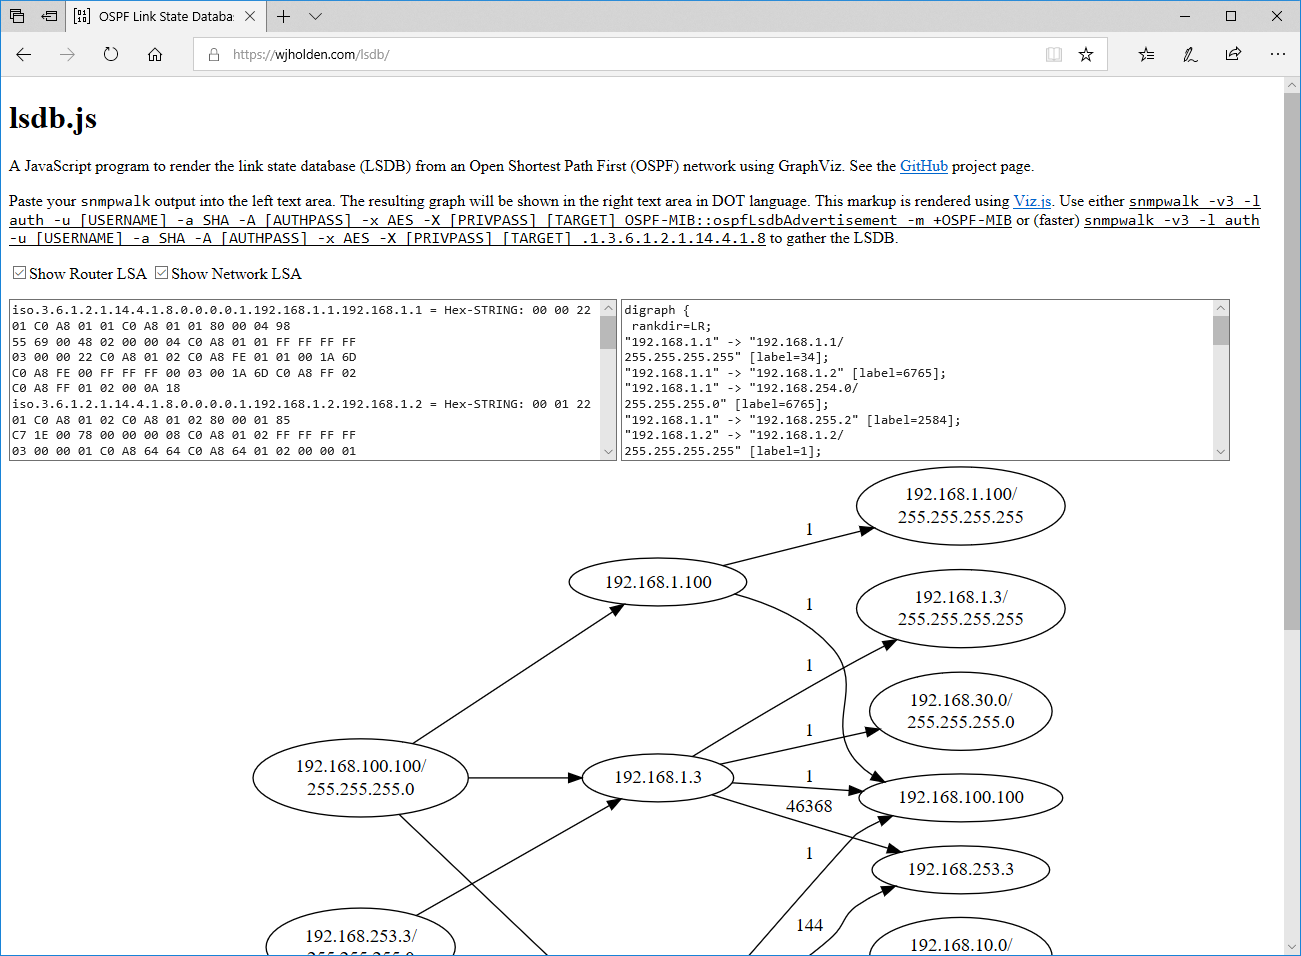
\includegraphics[width=\textwidth]{lsdb.PNG}
\caption{lsdb.js}
\label{fig:lsdb}
\end{figure}

lsdb.js is a derivative of an earlier Python program, Area Monitor (\url{https://github.com/wjholden/Area-Monitor}). Area Monitor began as an effort to peer with OSPF routers over IP protocol number 89. My first experiment with such low-level programming was in a C program (\url{https://github.com/wjholden/hello-ospf}). Low-level network programming is very difficult. After significant research and experimentation, I realized that you can get the LSDB in its entirety directly from a router using SNMP.

The \texttt{snmpwalk} command is an easy and useful method to gather the LSDB. Either of the following commands are sufficient to gather the LSDB over SNMPv3. Use the latter if the OSPF-MIB is not available to \texttt{snmpwalk}. lsdb.js consists of only four total files (one \texttt{.html} and three \texttt{.js}) that can be hosted as static content anywhere or viewed locally.

\begin{lstlisting}
snmpwalk -v3 -l auth -u [USERNAME] -a SHA -A [AUTHPASS] -x AES -X [PRIVPASS] [TARGET] OSPF-MIB::ospfLsdbAdvertisement -m +OSPF-MIB
snmpwalk -v3 -l auth -u [USERNAME] -a SHA -A [AUTHPASS] -x AES -X [PRIVPASS] [TARGET] .1.3.6.1.2.1.14.4.1.8
\end{lstlisting}

Paste the output from \texttt{snmpwalk} into the left text area.

lsdb.js translates the link state database to the DOT format used by GraphViz. The program can interpret router and network link state advertisements (LSAs). These LSAs may be switched on or off by toggling the checkboxes shown in the web page. The DOT output is shown in the second text area.

Finally, lsdb.js calls Viz.js (\url{http://viz-js.com/}), an emscripten (\url{https://emscripten.org}) build of Graphviz (\url{https://www.graphviz.org}), to render the DOT output as an image. This image is shown in the web page.

Operators may edit the text in both text areas to customize their graphic.

The layout of network diagrams is generally less than beautiful. The network diagrams generated might be useful to:

\begin{itemize}
	\item Get started with a network diagram. Assign vertices to subgraphs and manually adjust their ordering of the vertices to find an appealing arrangement.
	\item Change detection. Run \texttt{snmpwalk} as a scheduled task on a regular basis. Store the output for later use in ``spot-the-differences'' troubleshooting.
	\item Discover mismatched interface costs. An interesting design feature (design flaw?) of OSPF is that interface costs may be mismatched. For example, routers R1, R2, and R3 may each be connected to the same broadcast network, but their the \texttt{ip ospf cost} configuration can be unequal. Unequal link costs may cause asymmetric routing. Link costs are shown as edge labels.	
\end{itemize}

\section{Node Monitor}

\textbf{Location}: \url{https://github.com/wjholden/Node-Monitor}

\textbf{Input}: A list of hostnames or IP addresses to monitor as a file or as standard input.

\textbf{Output}: A table showing the reachability of each device (see figure \ref{fig:Node-Monitor}).

\textbf{Language}: Java

\begin{figure}[h]
\centering
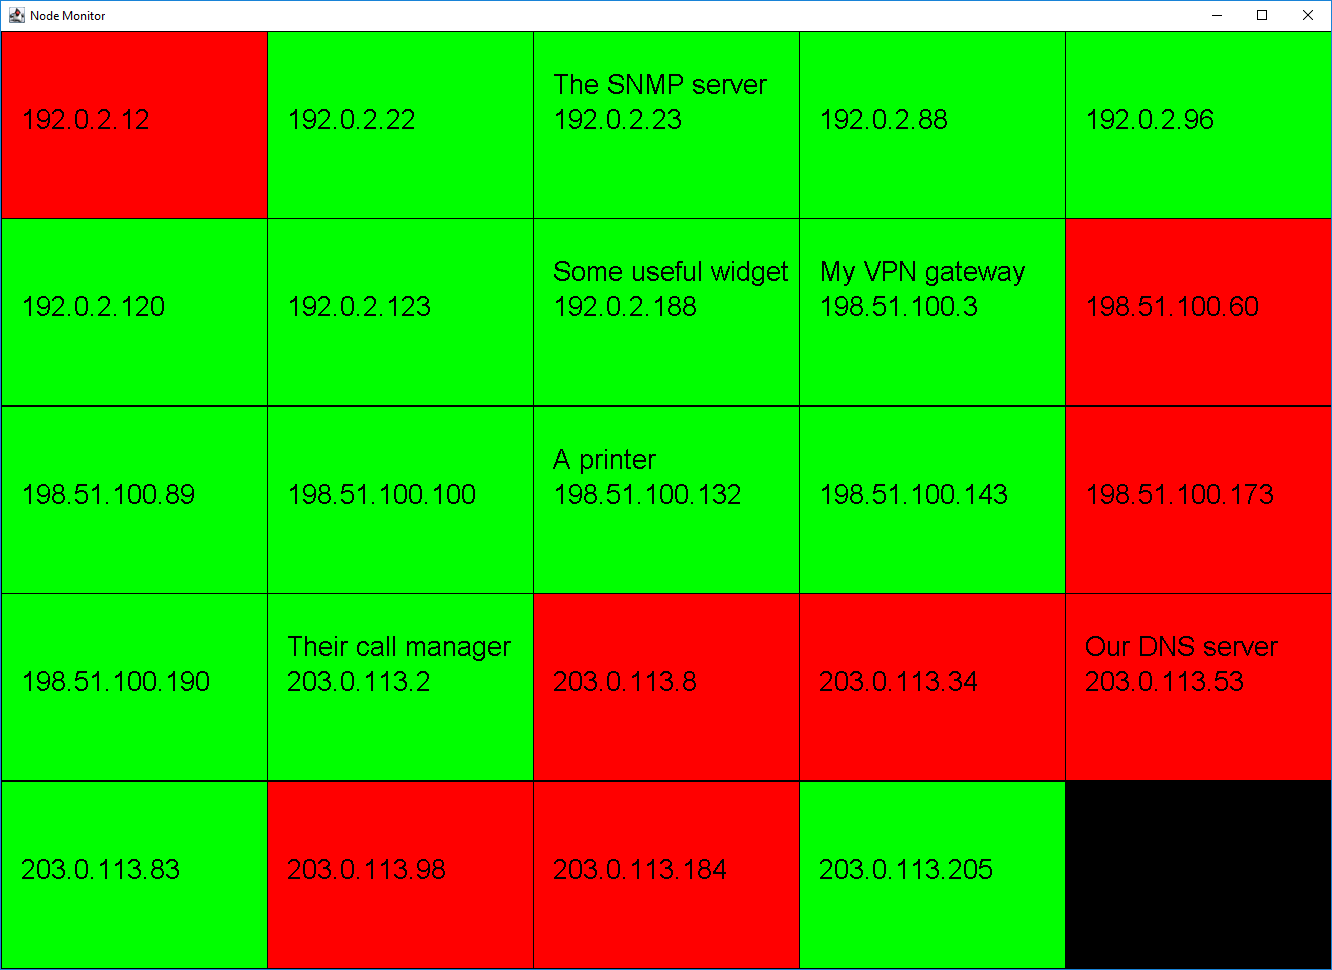
\includegraphics[width=\textwidth]{Node-Monitor}
\caption{Node Monitor}
\label{fig:Node-Monitor}
\end{figure}

Node Monitor is a simple pure-Java solution to ``ping'' network devices to test their availability. Technically, the method by which the IP addresses are polled is not specified. Reachability is determined by Java's \texttt{java.net.InetAddress.isReachable} method (see \url{https://docs.oracle.com/javase/8/docs/api/java/net/InetAddress.html}). Node Monitor has no third-party dependencies, requires no installation, and does not require superuser privileges.

Node Monitor's configuration can be supplied as a file or as standard input. The format is a list of lines containing one to four tab-separated columns. Only the first column is mandatory. The first column is the IP address or hostname to be polled.

The second column is the timeout, in seconds, that the system waits until considering a ping failed. If not specified, the timeout defaults to two seconds.

The third column is the frequency, in seconds, with which we poll the node. If not specified, the frequency defaults to thrice the timeout.

The final column is a textual description of the node.

If supplying this configuration as a file, simply provide the file name as the only command-line argument for the program. An example configuration is shown below:

\begin{lstlisting}
198.51.100.3	2	10	My VPN gateway
203.0.113.53	2	10	Our DNS server
192.0.2.23	5	30	The SNMP server
198.51.100.132	8	25	A printer
203.0.113.2	1	10	Their call manager
192.0.2.188	1	5	Some useful widget
198.51.100.60	2	10
203.0.113.205	2
192.0.2.88
\end{lstlisting}

Node Monitor is not at all novel. There are dozens, perhaps hundreds, of commercial and open network monitoring solutions that provide superior functionality and a more appealing interface. The value Node Monitor brings is its simplicity. Given only a list of hostnames or IP addresses, a system administrator can begin monitoring the availability of their network in seconds. Node Monitor automatically sorts nodes in reading order by the numerical value of their IP addresses. Node Monitor organizes nodes in a left-complete square.

To create an input file for Node Monitor, simply enter the desired IP addresses or hostnames into a text file. Save the file to the same folder as \texttt{Node\_Monitor.jar} and enter the command \texttt{java -jar Node\_Monitor.jar FILENAME.TXT}.

Node Monitor's graphical user interface is not at all polished. Use the + and - keys to increase and decrease the font size. Use arrow keys ($\uparrow\downarrow\leftarrow\rightarrow$) to position text. Press \texttt{f} to enter fullscreen and press \texttt{q} to quit. Fullscreen is known to not work on OpenJDK.

\section{Key Chain Generator} \label{sec:KeyChain}

\textbf{Location}: \url{https://wjholden.com/keychain}

\textbf{Input}: Number of years (1--10) of keys to generate.

\textbf{Output}: A key chain in the format Cisco IOS expects with three overlapping keys per year and one key (always key number 255) with an infinite lifetime (see figure \ref{fig:keychain}).

\textbf{Language}: JavaScript

\begin{figure}[h]
\centering
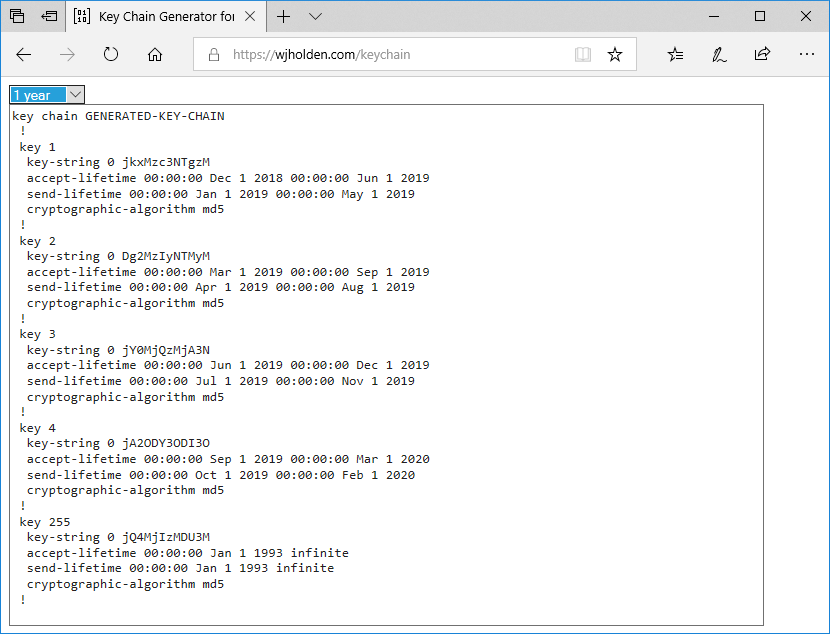
\includegraphics[width=\textwidth]{Key-Chain.PNG}
\caption{Key Chain Generator}
\label{fig:keychain}
\end{figure}

Network technicians should be familiar with using key chains to authenticate the Enhanced Interior Gateway Routing Protocol (EIGRP) and Open Shortest Path First (OSPF) dynamic routing protocols. Key chain-based authentication has some security advantages, but it can be tedious and difficult to create a ``perfect'' key chain with overlapping keys. The Key Chain Generator creates random keys that are accepted for a six month period but sent for only four months. Key lifetime overlap is intended to allow tolerance for clock drift. The infinite lifetime key is required in by security guidelines in some organizations.

Interestingly, the behavior of router authentication in Cisco's OSPF implementation is very different from its EIGRP implementation. According to \url{https://www.cisco.com/c/en/us/td/docs/ios-xml/ios/iproute_ospf/configuration/xe-3s/iro-xe-3s-book/iro-ospfv2-crypto-authen-xe.html}, ``OSPF selects the key that has the maximum life time'' and a ``key having an infinite lifetime is preferred.'' By contrast, \url{https://www.cisco.com/c/en/us/td/docs/ios-xml/ios/iproute_eigrp/configuration/xe-3s/ire-xe-3s-book/ire-rte-auth.html} states that in EIGRP ``the software examines the key numbers in the order from lowest to highest, and uses the first valid key that it encounters.'' The EIGRP behavior seems more closely aligned to one's expectations.

Those who modify this software or its output should avoid using keys numbered 0 or anything greater than 255 if using OSPF. OSPF includes an eight-bit key ID in its authentication field (\url{https://tools.ietf.org/html/rfc2328#appendix-D}). Cisco's IOS will send key 0 as default (empty) key if the configuration is incomplete and will log a \texttt{OSPF-4-INVALIDKEY} warning if received (see \url{https://packetlife.net/blog/2010/jun/1/ospfv2-authentication-confusion/}).

\section{CommSync II Output Interpreter}

\textbf{Location}: \url{https://wjholden.com/commsync}

\textbf{Input}: 

\textbf{Output}: 

\textbf{Language}: JavaScript

The organization I worked for from 2017--2019 operates CommSync II devices (``CommSync'').
The CommSync is a GPS and atomic clock which provides timing.
Younger network technicians may be surprised to learn that timing was a major consideration in the planning and operation of telecommunications.
The CommSync devices serve as an external time reference 


\end{document}